\graphicspath{{Notes/Figs/}}
OS Name: Microsoft Windows 10 Home

OS version: 10.0.19042 Build 19042

Processor:	Intel(R) Core(TM) i7-5500U CPU @ 2.40GHz, 2401 Mhz, 2 Core(s), 4 Logical Processor(s)

Modelica library version: 3.2.3

OpenModelica v1.17.0 (64-bit)

OMSimulator v2.0.0.post284-gc8ec782-mingw


\section{Modelica}
Modelica is a language for modeling of physical systems, designed to support effective library development and model exchange. It is a modern language built on acausal modeling with mathematical equations and object-oriented constructs to facilitate reuse of modeling knowledge %\cite{ModelicaUnifiedObjectOriented}
. Coding with such a language let any developer to create a faithful model to reality of any kind, thanks to the continuous updates of the Modelica Libraries% \cite{ModelicaLibrariesModelica}
 thanks to the work of both the \textit{Modelica Association} and users development. The Modelica Libraries are a collection of free and commercial libraries which largely covers multiple simulation domains: with the use of these libraries it is possible to model systems which belong to magnetic, electrical, mechanic, fluid and thermal domains with the reliability of using standardized libraries %\cite{ModelicaStandardLibrary2021}
 and with the possibility of simulating multi-domain systems to effectively study the behavior of each component of the model.
% and at the same time being able to modify them to adapt them to the model that needs to be created.

There are specific semantic restrictions for a simulation model to ensure that the model is complete; they allow its flat Modelica structure to be further transformed into a set of differential, algebraic and discrete equations (= flat hybrid DAE), which consists in:

\begin{itemize}
\itemsep 0em
\item Declarations of variables with the appropriate basic types, prefixes and attributes, such as ”\small{\texttt{\textcolor{red}{parameter} \textcolor{red}{Real} v = 5}}”.
\item Equations from equation sections.
\item Function invocations where an invocation is treated as a set of equations which involves all input and all result variables (number of equations = number of basic result variables).
\item Algorithm sections where every section is treated as a set of equations which involves the variables occurring in the algorithm section (number of equations = number of different assigned variables).
\item When-clauses where every when-clause is treated as a set of conditionally evaluated equations, also called instantaneous equations, which are functions of the variables occurring in the clause (number of equations = number of different assigned variables).
\end{itemize}

Modeling with such a language could decrease the modeling time of a system and improve the analysis part of the process. 

\subsection{OMEdit}
Interface description:
\begin{itemize}
\itemsep 0em
\item Windows Browsers
	\begin{itemize}
	\itemsep 0em
	\item Libraries Browser
	\item Documentation Browser
	\item Variables Browser
	\item Messages Browser
	\end{itemize}
\item Perspectives
	\begin{itemize}
	\itemsep 0em
	\item Welcome Perspective
	\item Modeling Perspective
		\begin{itemize}
		\itemsep 0em
		\item Icon view
		\item Diagram view
		\item Text view
		\item Documentation view
		\end{itemize}
	\item Plotting Perspective
	\item Debugging Perspective
	\end{itemize}
\end{itemize}

Toolbar: 
\begin{figure}[H]
 \centering
 
\includegraphics[width=\textwidth]{toolbar}
 \caption{OMEdit toolbar}
 \label{fig:omedit_toolbar}
\end{figure}

Simulation procedure:
\begin{itemize}
\itemsep 0em
\item Check model
\item Simulation setup
\item Simulate (with Transformation Debugger, with Algorithmic Debugger, with Animation)
\end{itemize}
\section{RRRR planar loop}
Planar loop in OpenModelica is made of 4 components of the Modelica > Mechanics > Multibody package of the Modelica library :
\begin{itemize}
\itemsep 0em
\item \textit{World}: represents a global coordinate system fixed in ground mainly used as inertial system and to define the gravity field.
\item \textit{BodySahpe}: defines a rigid body with mass and inertia tensor.
\item \textit{Revolute}: defines a revolute joint which can be driven by a mechanical flange
\item \textit{RevolutePlanarLoopConstraint}: when a planar loop is modeled, this particular revolute component revoves 3 of the 5 contraints given to the system by a normal revolute joint and make the system mathematically solvable by the symbolic solver.
\end{itemize}
The compete description of each component can be found in 
The final shape of the model is the one show in Fig. \ref{fig:rrrr_planarLoop}

\begin{figure}[H]
 \centering
 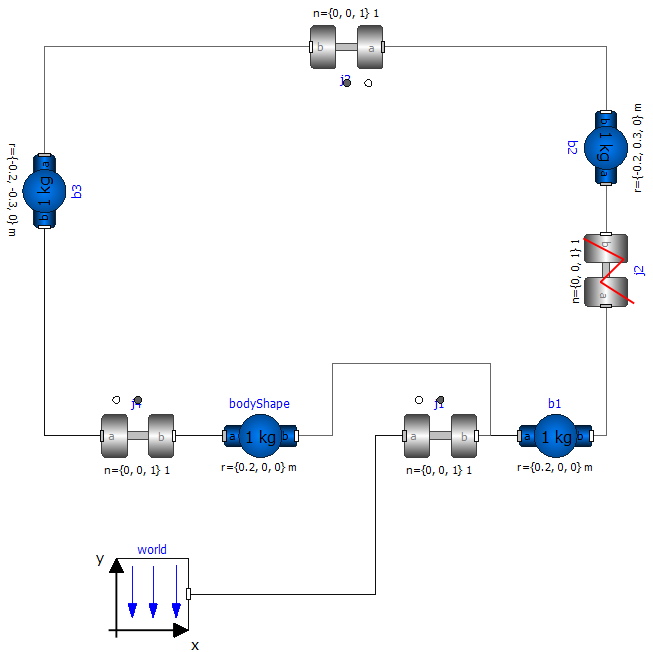
\includegraphics[width=0.7\textwidth]{rrrr_closedloop_model}
 \caption{Modelica model of a 4 bar RRRR planar loop}
 \label{fig:rrrr_planarLoop}
\end{figure}